\documentclass[12pt]{beamer}
\usetheme{amcg}
\beamertemplatenavigationsymbolsempty
\renewcommand{\thefootnote}{}
\providecommand{\e}[1]{\ensuremath{\times 10^{#1}}}
\usepackage{mathptmx}
\usepackage{helvet}
\newcommand\TILDE{\char`\~}
\usepackage{listings}

% items enclosed in square brackets are optional; explanation below
\title[Code Generation]{Automated Code Generation in Fluidity}
\subtitle[]{}
\institute{}
\author[Christian Jacobs]{\large{Christian Jacobs}}
\date{}

\begin{document}

%--- the titlepage frame -------------------------%
\begin{frame}
  \titlepage
\end{frame}

\begin{frame}
    \frametitle{Background}
\begin{itemize}
    \item The core of Fluidity comprises \textcolor{red}{low-level}, \textcolor{red}{hand-written} Fortran code to assemble the system of equations.
    \item This is typically \textcolor{red}{sub-optimal} and does not cater for \textcolor{red}{different hardware}, e.g. GPUs, AVX, ...
    \item We would need to \textcolor{red}{re-engineer} the hand-written code and throw in a few calls to CUDA, OpenCL or some other backend.
    \item This places \textcolor{red}{extra burden} on the developer to not only be an expert in numerical methods and their application area, but also an expert in software engineering and parallelisation.
\end{itemize}
\end{frame}

\begin{frame}
    \frametitle{Firedrake}
\begin{itemize}
    \item \textcolor{red}{Firedrake} (www.firedrakeproject.org) is a library which generates the assembly code \textcolor{red}{automatically}.
    \item Problems are specified in a high-level, near-mathematical, Python-based language called \textcolor{red}{UFL}...
    \item ...and then \textcolor{red}{compiled down} into optimised, low-level \textcolor{red}{C code} that is \textcolor{red}{targetted} towards a desired backend (MPI, MPI+OpenMP, CUDA, OpenCL, ...).
\end{itemize}
\end{frame}

\begin{frame}
    \frametitle{Re-engineering}
\begin{itemize}
    \item We are in the process of re-engineering Fluidity to use Firedrake's automated code generation techniques.
    \item Models and numerical schemes are being \textcolor{red}{ported over} from Fortran to UFL.
\end{itemize}
\end{frame}

\begin{frame}
    \frametitle{}
\begin{center} 
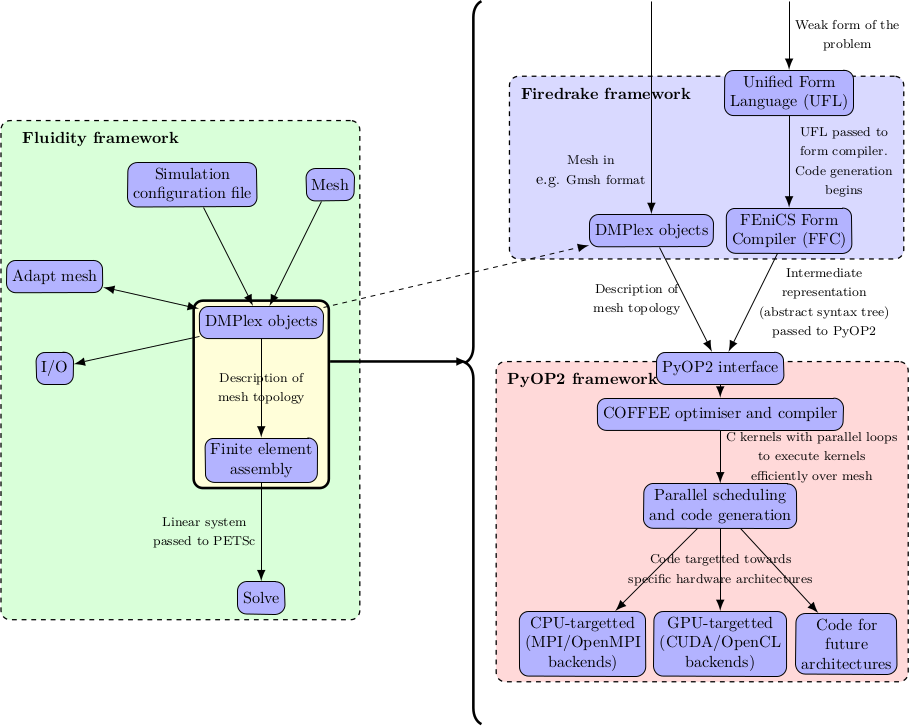
\includegraphics[width=0.85\textwidth]{images/assembly_replacement.png} 
\end{center}
\end{frame}

\begin{frame}
    \frametitle{Firedrake-Fluids}
\begin{itemize}
    \item A prototype for the `new Fluidity' code which uses code generation, called \textcolor{red}{Firedrake-Fluids}, is available at: \texttt{github.com/firedrakeproject/firedrake-fluids}
    \item Currently only the \textcolor{red}{shallow water} model has been implemented in UFL, along with SU stabilisation and an LES turbulence model.
\end{itemize}
\end{frame}

\begin{frame}
    \frametitle{Using Code Generation}
\begin{itemize}
    \item Convert the old-style options file used with the `hand-written' model to a `new-style' one is compatible with the Firedrake-based model:
    \item \texttt{python tools/fl2ff.py old.flml new.swml}
    \item Execute the Firedrake-based model with the Python interpreter:
    \item \texttt{python firedrake\_fluids/shallow\_water.py new.swml}
\end{itemize}
\end{frame}

\end{document}
